\input ../preamble

\begin{document}

{\Huge


\centerline{\bf TTIC 31230, Fundamentals of Deep Learning}
\bigskip
\centerline{David McAllester, April 2017}

\vfill
\centerline{\bf Regularization}
\vfill
\vfill
\centerline{Over-Parameterization}
\vfill
\centerline{Weight Decay}
\vfill
\centerline{Dropout}
\vfill
\centerline{Early Stopping}
\vfill
\centerline{PAC-Bayesian Learning Theory}

\vfill
\centerline{}
\slide{Over-Parameterization}

If we have more parameters than data then we can fit any set of labels.

\vfill
\begin{quotation}
``Our experiments establish that state-of-the-art convolutional networks
for image classification trained with stochastic gradient methods easily fit a random
labeling of the training data.''
\end{quotation}

\vfill
\rightline{Rethinking Generalization, Zhang et al., ICLR 2017}

\slide{Over-Parameterization}

Inception (Google's net) on CIFAR10 can fit random labels on the training data.

\vfill
\centerline{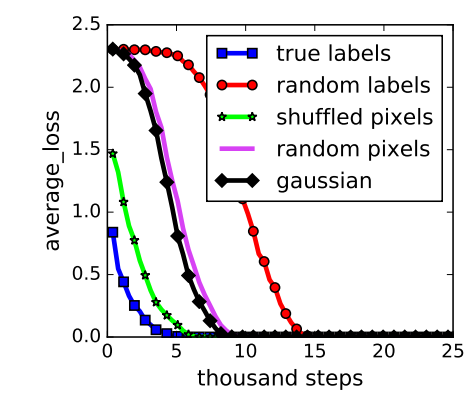
\includegraphics[width = 5in]{../images/RandomLabels1}}

\slide{Using Fewer Parameters :)}

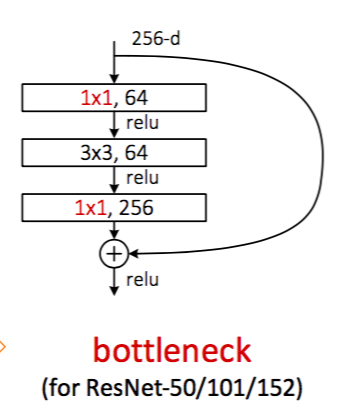
\includegraphics[height= 4.5in]{../images/bottleneck} \begin{minipage}[b]{2in}

$$2 \times 256 \times 64 \;+ \;9 \times 64 \times 64 = 69,632$$

  \bigskip
  \bigskip
  $$9 \times 256 \times 256 = 589,824$$
  \bigskip
  \bigskip
    \bigskip
  \bigskip
  \bigskip
  \bigskip
    \bigskip
  \bigskip
\end{minipage}

\centerline{\huge [Kaiming He]}

\slide{Early Stopping}

During SGD one should be tracking validation loss and validation error.

\vfill
A typical stopping rule (on a GPU) is to stop training when the validation error has not improved for two or three consecutive epochs.

\slide{Early Stopping}

\centerline{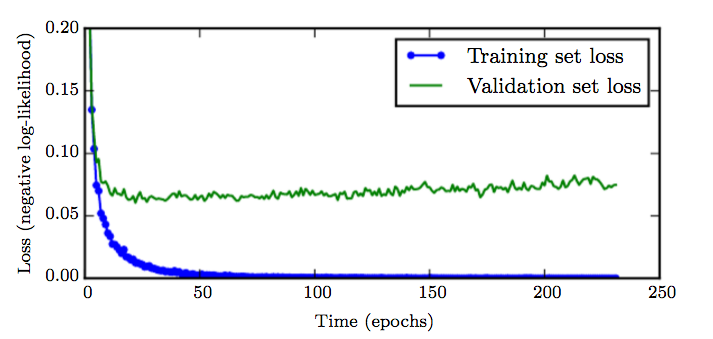
\includegraphics[width = 8in]{../images/EarlyStopping}}

\centerline{[Goodfellow et al.]}

\slide{Early Stopping}

\centerline{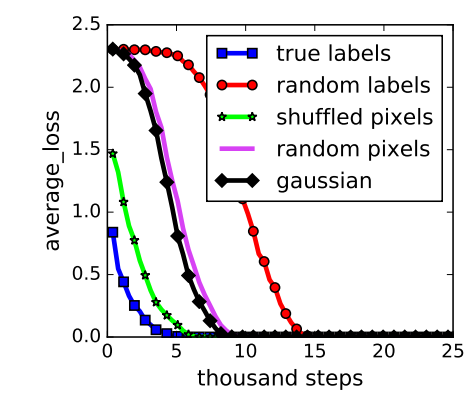
\includegraphics[width = 4in]{../images/RandomLabels1}}

\slide{$L_2$ Regularization (Weight Decay)}

Impose a prior probability on parameters 

\vfill
$$P(\Phi) \propto e^{-\frac{1}{2}||\Phi||^2}$$

\vfill
This can be used to justify $L_2$ regularization (ridge regression is a special case).

\vfill
$$\Phi^* = \argmin_\Phi \;E_{(x,y) \sim \mathrm{Train}}\;\mathrm{loss}(\Phi,x,y) + \frac{1}{2}\lambda||\Phi||^2$$

\vfill
PAC-Bayesian theory (and other theory) can be used to show that a small value of this regularized optimization objective guarantees generalization independent of any truth of the prior (more later).

\slide{Weight Decay}

\begin{eqnarray*}
  & & \nabla_\Phi \;\left(E_{(x,y) \sim \mathrm{Batch}}\;\mathrm{loss}(\Phi,x,y) + \frac{1}{2}\lambda||\Phi||^2\right) \\
  \\
  & = & \Phi.\mathrm{grad} + \lambda \Phi \\
  \\
  \Phi^{t+1} & = & \Phi^t - \eta \Phi.\mathrm{grad} - \gamma \Phi^t
\end{eqnarray*}

\vfill
$-\gamma \Phi$ is called weight decay where $\gamma$ is the weight decay parameter. 

\vfill
Warning: PyTorch does $+\gamma\Phi$ rather than $-\gamma\Phi$ and it seems to be standard for the decay parameter to be negative {\large \tt :P}

\ignore{
\slide{Test Error as a Function of Training Label Corruption}

\centerline{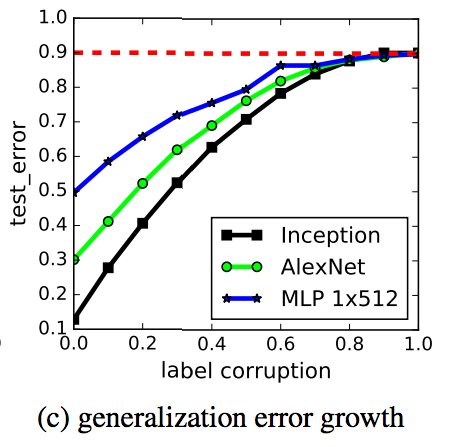
\includegraphics[width = 5in]{../images/RandomLabels2}}
}

\slide{Implicit Regularization}

Consider solving linear least squares regression with SGD.

\vfill
SGD maintains the invariant that $\Phi$ is a linear combination of input vectors.

\vfill
When over-parameterized the input vectors span a proper subspace.

\vfill
For least squares regression, SGD finds the zero training error solution minimizing $||\Phi||$.

\vfill
But driving the training error to zero is often a mistake.


\slide{Dropout}

Dropout can be viewed as an ensemble method.


\vfill
To draw a model from the ensemble we randomly select a mask $\mu$ with

$$\left\{\begin{array}{ll} \mu_i = 0 & \mbox{with probability $\alpha$} \\ \\ \mu_i = 1 & \mbox{with probability $1-\alpha$}
\end{array}\right.$$

\vfill
Then we use the model $(\Phi,\;\mu)$ with weight layers defined by


\vfill
$$y_i = \mathrm{Relu}\left(\sum_j\;W_{i,j} \;\mu_jx_j\right)$$

\slide{Dropout Training}

Repeat:

\vfill

\begin{itemize}
\item Select a random dropout mask $\mu$
  
\vfill
\item $\Phi \;\minuseq\; \nabla_\Phi\; \ell(\Phi, \mu)$
\end{itemize}

\vfill
Backpropagation must use the same mask $\mu$ used in the forward computation.

\slide{Test Time Scaling}


\vfill
At train time we have

\vfill
$$y_i = \mathrm{Relu}\left(\sum_j\;W_{i,j} \;\mu_j x_j\right)$$


\vfill
At test time we have

\vfill
$$y_i = \mathrm{Relu}\left((1-\alpha)\;\sum_j\;W_{i,j} \;x_j\right)$$

\vfill
At test time we use the ``average network''.

\slide{Dropout for Least Squares Regression}

Consider simple least square regression

\begin{eqnarray*}
  \Phi^* & = &  \argmin_\Phi\;\; \mathrm{E}_{(x,y)} \;\expectsub{\mu}{(y - \Phi \cdot (\mu \odot x))^2} \\
  \\
  & = & \expect{(\mu\odot x)(\mu\odot x)^{\top}}^{-1}\; \expect{y (\mu\odot x)} \\
  \\
  & = & \argmin_\Phi\;\; \mathrm{E}_{(x,y)} (y - (1-\alpha) \Phi \cdot x)^2 + \sum_i\frac{1}{2}(\alpha - \alpha^2) \expect{x_i^2} \Phi_i^2
\end{eqnarray*}

\vfill
In this case dropout is equivalent to a form of $L_2$ regularization --- see Wager et al. (2013).

\slide{Search Over Regularization Parameters}

Hyper-parameter search on Penn Tree Bank Language Modeling with a 4 layer LSTM.

\centerline{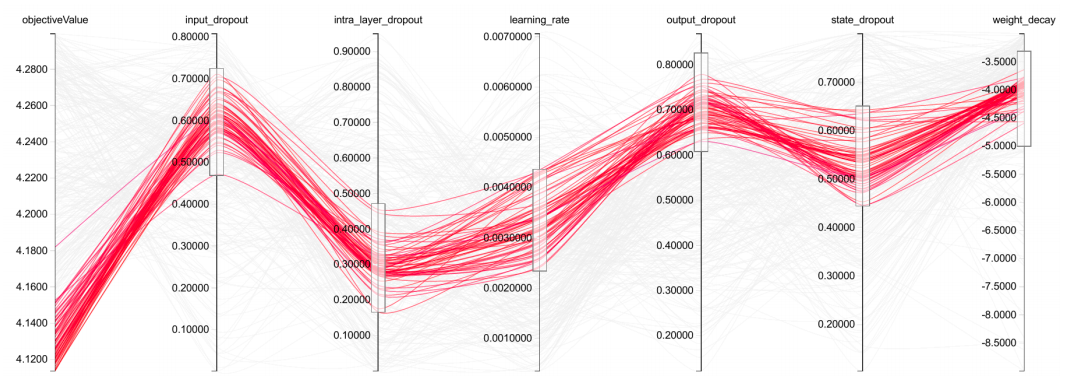
\includegraphics[width = 7in]{../images/HyperSearch}}
\centerline{\large ~ \hspace{3em} Loss \hspace{2em} Input Drop \hspace{1em} Intra Lay Drop \hspace{1em} Learning Rate \hspace{1em} Output Drop \hspace{1em}  State Drop \hspace{1em} Weight Decay}

\centerline{Melis et al. 2017.}

Following Gal and Ghahrmani 2016, state dropout is an RNN parameter dropout with the same mask across the sequence.

\slide{Early Stopping}

Early stopping can limit $||\Phi||$ --- growing a large $||\Phi||$ can take a long time.

\vfill
Early stopping seems more related to limiting $||\Phi - \Phi_\mathrm{init}||$
\vfill

Theoretical guarantees work for $||\Phi - \Phi_{\mathrm{init}}||^2$ just as well as for $||\Phi||^2$.

\vfill
This suggests replacing weight decay with

\vfill
$$\Phi^{t+1} = \Phi^t - \eta \Phi.\mathrm{grad} - \gamma(\Phi - \Phi_\mathrm{init})$$

\ignore{
  The following slide is not true --- gradient flow approaches the optimum directly along the smallest eigenvector of H.  The regularization path
  satisfies g = lambda(t) Phi and approaches with a fixed nonzero angle to the eigenvector.
  
\slide{Early Stopping}

\centerline{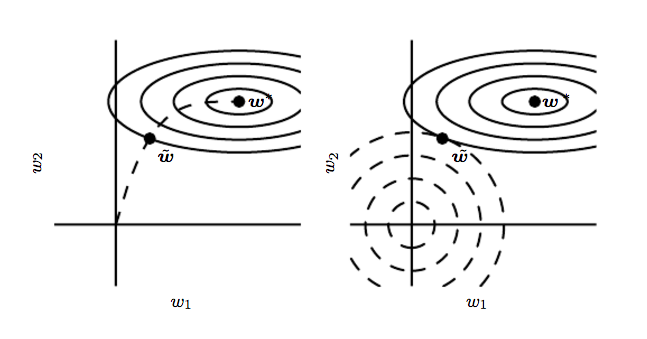
\includegraphics[width = 7in]{../images/EarlyStopping2}}
\centerline{[Goodfellow et al.]}

\vfill
For differential Newton updates (gradient flow) on a quadratic loss function, with $\Phi$ initialized to zero, early stopping and $L_2$ regularization are equivalent.
}

\slide{Learning Theory: Nature vs. Nurture}

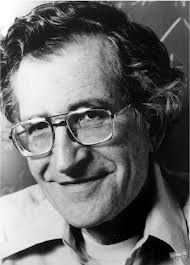
\includegraphics[width=1.0 in]{../images/Chomsky} \begin{minipage}[b]{8in} Noam Chomsky: 
Natural language grammar is unlearnable without with an innate linguistic capacity. This position is supported by the ``no free lunch theorem''.\end{minipage}

\vfill
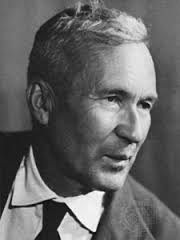
\includegraphics[height=1.0 in]{../images/Kolmogorov}
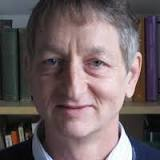
\includegraphics[height=1.0 in]{../images/Hinton}
\begin{minipage}[b]{7in}
Andrey Kolmogorov, Geoff Hinton: Universal learning algorithms exist. This position is supported by the ``free lunch theorem''.
\end{minipage}

\slide{The No Free Lunch Theorem}

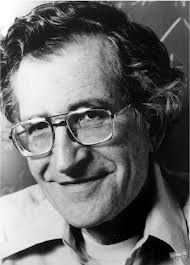
\includegraphics[width=1.0 in]{../images/Chomsky} 

Without prior knowledge, such as universal grammar, it is impossible to make a prediction for an input you have not seen in the training data.


\vfill
{\bf Proof:} Select a predictor $h$ uniformly at random from all functions from ${\cal X}$ to ${\cal Y}$ and then take the data distribution to draw pairs $(x, h(x))$
where $x$ is drawn uniformly from ${\cal X}$.  No learning algorithm can predict $h(x)$ where $x$ does not occur in the training data.

\slide{The Free Lunch Theorem}

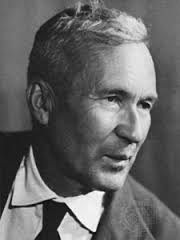
\includegraphics[height=1.0 in]{../images/Kolmogorov}
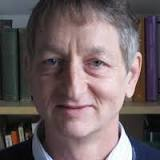
\includegraphics[height=1.0 in]{../images/Hinton}

Universal (knowledge-free) learning algorithms exists.

\vfill
Let $h$ be a C++ procedure taking an input from ${\cal X}$ and returning a value in ${\cal Y}$, where $h$ is written using calls to prodecures in an (arbitrarily large) code library $L$.
Let $|h|$ be the number of bit in a standard compression algorithm applied to the source code for $h$.  We are compressing only the ``main'' procedure $h$ and not the library $L$.

\slide{The Free Lunch Theorem}

Consider a loss function $\mathrm{loss}(p,x,y)$ such that for any $C$ program $p$ and pair $(x,y)$ we have
$\mathrm{loss}(p,x,y) \in (0,L_\mathrm{max})$.

\vfill
    {\bf Theorem:} For any standard library $L$ fixed before the draw of the training data, we have that with probability
    at least $1-\delta$ over the draw of the training data the following holds {\em simultaneously} for all main programs $p$
    and $\lambda > 1/2$.
    \begin{eqnarray*}
      & & E_{(x,y)\sim \mathrm{Population}}\;\mathrm{loss}(p,x,y) \\
      \\
      & \leq & \frac{1}{1-\frac{1}{2\lambda}}\parens{E_{(x,y) \sim \mathrm{Train}}\;\mathrm{loss}(p,x,y)
          + \frac{\lambda L_\mathrm{max}}{N}\parens{(\ln 2)|h| + \ln\frac{1}{\delta}}}
      \end{eqnarray*}

\slide{PAC-Bayesian Generalization Bounds}

The free lunch theorem is a special case of a PAC-Bayesian generalization bound.

\vfill
PAC-Bayesian theory was introduced by me in 1999. The bounds have evolved over time
with contributions by Langford, Blum, Shawe-Taylor, Catoni and others.

\vfill
These bounds are of increasing interest today because of their applicability to deep networks.

\slide{A More General Free Lunch Theorem}

Let ${\cal H}$ be a discrete (countable) hypothesis class.  ${\cal H}$ might be the collection of all C programs.

\vfill
Let $P$ be a ``prior'' probability distribution on ${\cal H}$.  $P(h)$ might be $2^{-8|h|}$ where $|h|$ is the length of $h$ in bytes.

\vfill
\begin{eqnarray*}
  & & E_{(x,y)\sim \mathrm{Population}}\;\mathrm{loss}(h,x,y) \\
  \\
  & \leq & \frac{1}{1-\frac{1}{2\lambda}}\parens{E_{(x,y) \sim \mathrm{Train}}\;\mathrm{loss}(h,x,y)
    + \frac{\lambda L_\mathrm{max}}{N}\parens{\ln\frac{1}{P(h)} + \ln\frac{1}{\delta}}}
\end{eqnarray*}

\slide{A Finite Precision Corollary}

Suppose that we parameterize a classifier with a parameter vector $\Phi$ with $d$ parameters and use $b$ bits per parameter.

\vfill
\begin{eqnarray*}
  & & E_{(x,y)\sim \mathrm{Population}}\;\mathrm{loss}(\Phi,x,y) \\
  \\
  & \leq & \frac{1}{1-\frac{1}{2\lambda}}\parens{E_{(x,y) \sim \mathrm{Train}}\;\mathrm{loss}(\Phi,x,y)
    + \frac{\lambda L_\mathrm{max}}{N}\parens{(\ln 2)db + \ln\frac{1}{\delta}}}
\end{eqnarray*}

\slide{Proof}
$$L(h) = E_{(x,y)\sim \mathrm{Pop}}\;\mathrm{loss}(h,x,y)$$

\vfill
$$\hat{L}(h) = E_{(x,y)\sim \mathrm{Train}}\;\mathrm{loss}(h,x,y)$$

\slide{Proof}

Consider $\lmax = 1$ and define $\epsilon(h)$ by

\vfill
$$\epsilon(h) = \sqrt{\frac{2L(h)\parens{\ln\frac{1}{P(h)} + \ln\frac{1}{\delta}}}{N}}.$$

\vfill
By the relative Chernoof bound we have

\vfill
$$P_{\mathrm{Train} \sim \mathrm{Pop}}\parens{\hat{L}(h) \leq L(h) - \epsilon(h)} \leq e^{-N\frac{\epsilon(h)^2}{2L(h)}} = \delta P(h).$$

\slide{Proof}

$$P_{\mathrm{Train} \sim \mathrm{Pop}}\parens{\hat{L}(h) \leq L(h) - \epsilon(h)} \leq \delta P(h).$$

\vfill
$$P_{\mathrm{Train} \sim \mathrm{Pop}}\parens{\exists h\;\hat{L}(h) \leq L(h) - \epsilon(h)} \leq \sum_h \delta P(h) =\delta$$

\vfill
$$P_{\mathrm{Train} \sim \mathrm{Pop}}\parens{\forall h\;L(h) \leq \hat{L}(h) + \epsilon(h)} \geq 1- \delta$$

\slide{Proof}

$$L(h) \leq \widehat{L}(h) + \sqrt{L(h)\parens{\frac{2\parens{\ln\frac{1}{P(h)} + \ln\frac{1}{\delta}}}{N}}}$$

using
$$\sqrt{ab} = \inf_{\lambda > 0}\;\frac{a}{2\lambda} + \frac{\lambda b}{2}$$
\vfill
we get
$$L(h) \leq \widehat{L}(h) + \frac{L(h)}{2\lambda} + \frac{\lambda\parens{\ln\frac{1}{P(h)} + \ln\frac{1}{\delta}}}{N}$$

\slide{Proof}
$$L(h) \leq \widehat{L}(h) + \frac{L(h)}{2\lambda} + \frac{\lambda\parens{\ln\frac{1}{P(h)} + \ln\frac{1}{\delta}}}{N}$$

\vfill
Solving for $L(h)$ yields

\vfill
$$L(h) \leq \frac{1}{1-\frac{1}{2\lambda}}\parens{\hat{L}(h) + \frac{\lambda\lmax}{N}\parens{\ln \frac{1}{P(h)} + \ln \frac{1}{\delta}}}$$

\slide{A KL Divergence Bound}

Let $P$ be any ``prior'' and $Q$ be any ``poterior'' on any model space.

\vfill
Define
\begin{eqnarray*}
  L(Q) & =  &\expectsub{h \sim Q}{L(h)} \\
  \\
  \hat{L}(Q) & =  &\expectsub{h \sim Q}{\hat{L}(h)}
\end{eqnarray*}


\vfill
For any $P$ and any $\lambda > \frac{1}{2}$, with probability
at least $1-\delta$ over the draw of the training data, the following holds simultaneously for all $Q$.
\vfill
$$L(Q) \leq \frac{1}{1-\frac{1}{2\lambda}}\parens{\hat{L}(Q) + \frac{\lambda \lmax}{N}\parens{KL(Q,P) + \ln \frac{1}{\delta}}}$$

\slide{$L_2$ Bounds}

\vfill
\begin{eqnarray*}
P(w) & = & {\cal N}(0,1)^d \\
  \\
L(Q_\Theta) & = & \expectsub{\epsilon \sim {\cal N}(0,1)^d}{L(\Theta+\epsilon)} \\
\\
\hat{L}(Q_\Theta) & = & \expectsub{\epsilon \sim {\cal N}(0,1)^d}{\hat{L}(\Theta+\epsilon)}
\end{eqnarray*}

\vfill
\begin{eqnarray*}
  KL(Q_\Theta,P) & = & \frac{1}{2}||\Theta||^2 \\
  \\
  L(Q_\Theta) & \leq & \frac{1}{1-\frac{1}{2\lambda}}\parens{\hat{L}(Q_\Theta) + \frac{\lambda \lmax}{N}\parens{\frac{1}{2}||\Theta||^2 + \ln \frac{1}{\delta}}}
\end{eqnarray*}

\slide{A Dropout Bound}

\begin{eqnarray*}
KL(Q_{\alpha,\Phi},\;Q_{\alpha,0}) & = & \expectsub{\mu \sim P_\alpha, \epsilon \sim {\cal N}(0,1)^d}
{\ln \frac{P_\alpha(\mu) e^{-\frac{1}{2}||\mu \odot \epsilon||^2}}{P_\alpha(\mu) e^{-\frac{1}{2}||\mu \odot (\Phi + \epsilon)||^2}}} \\
\\
& = & \expectsub{\mu \sim P_\alpha}{\frac{1}{2}||\mu \odot \Phi||^2} \\
\\
& = & \frac{1-\alpha}{2}||\Phi||^2
\end{eqnarray*}

$$L(Q_{\alpha,\Phi}) \leq \frac{1}{1-\frac{1}{2\lambda}}\parens{\hat{L}(Q_{\alpha,\Phi}) + \frac{\lambda \lmax}{N}\parens{\frac{1-\alpha}{2}||\Phi||^2 + \ln \frac{1}{\delta}}}$$

\slide{$L_2$ PAC-Bayesian Bounds in Action}

Computing Nonvacuous Generalization Bounds for Deep (Stochastic) Neural Networks with Many More Parameters than Training Data, (Dziugaite and Roy, arXiv, 2017)

\vfill
\centerline{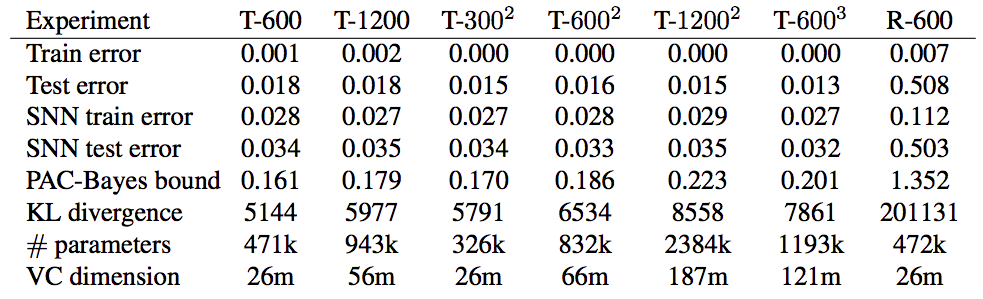
\includegraphics[width = 8in]{../images/Roy}}

\vfill
{\bf The bounds are based on $L_2$ distance of the weight vector to the initialization.}

\vfill
{\bf The weight vector is retrained to minimize the bound.}


\slideplain{A Formal Definition of Implicit Prior}

We now consider any learning algorithm ${\cal A}$ which takes training data
and returns a probability distribution $Q_{\cal A}(\mathrm{Train})$ on parameters.

\vfill
define $Q_{\cal A}(\mathrm{Pop}) = E_{\mathrm{Train} \sim \mathrm{Pop}}\;Q_{\cal A}(\mathrm{Train})$

\vfill
To draw $\Phi$ from $Q_{\cal A}(\mathrm{Pop})$ I first draw $\mathrm{Train}$ from $\mathrm{Pop}$ and then draw $\Phi$ from $Q_A(\mathrm{Train})$.

\vfill
We will show that $Q_{\cal A}(\mathrm{Pop})$ is an optimal prior for ${\cal A}$ running on $\mathrm{Pop}$.  We can think of $Q_{\cal A}(\mathrm{Pop})$
as an implicit prior for ${\cal A}$.

\slide{Optimality of $Q_{\cal A}(\mathrm{Pop})$}

Consider an arbitrary prior $P$.

\vfill
\begin{eqnarray*}
  & & E_{\mathrm{Train}\sim\mathrm{Pop}}\;KL(Q_{\cal A}(\mathrm{Train}),P) \\
  \\
  & = & E_{\mathrm{Train}\sim\mathrm{Pop}}\;\ln \frac{Q_{\cal A}(\mathrm{Train})(h)}{P(h)}  \\
\\
\\
& = & \expectsub{\mathrm{Train}\sim \mathrm{Pop},\;h \sim Q_{\cal A}(\mathrm{Train})}{\ln \frac{Q_{\cal A}(\mathrm{Train})(h)}{Q_{\cal A}(\mathrm{Pop})(h)}} \\
\\
\\
& & + \expectsub{h \sim Q_{\cal A}(\mathrm{Pop})}{\ln \frac{Q_{\cal A}(\mathrm{Pop}(h))}{P(h)}}
\end{eqnarray*}

\slideplain{Optimality of $Q_{\cal A}(\mathrm{Pop})$}

\begin{eqnarray*}
  & & E_{\mathrm{Train}\sim\mathrm{Pop}}\;KL(Q_{\cal A}(\mathrm{Train}),P) \\
\\
& = & \expectsub{\mathrm{Train}\sim \mathrm{Pop}}{KL(Q_{\cal A}(\mathrm{Train}),Q_{\cal A}(\mathrm{Pop}))} + KL(Q_{\cal A}(\mathrm{Pop}),P)
\end{eqnarray*}

\vfill
So $Q_{\cal A}(\mathrm{Pop})$ is an {\bf optimal prior} (or {\bf implicit prior}) for algorithm ${\cal A}$.

\slide{An Implicit Prior Generalization Bound}

For any given learning algorithm ${\cal A}$ and $\lambda > \frac{1}{2}$ we have the following with probability at least $1-\delta$ over the draw of the training data.

\vfill
\begin{eqnarray*}
  & & L(Q_{\cal A}(\mathrm{Train})) \\
  \\
  & \leq &\frac{1}{1-\frac{1}{2\lambda}}\parens{\begin{array}{l}\hat{L}(Q_{\cal A}(\mathrm{Train})) \\ \\
    + \frac{\lambda\lmax}{N}\parens{KL(Q_{\cal A}(\mathrm{Train}),Q_{\cal A}(\mathrm{Pop})) + \ln \frac{1}{\delta}} \end{array}}
\end{eqnarray*}

\ignore{
\slide{The Broad Basin Hypothesis}

Do broad basins in the loss function generalize better?

\vfill

{\bf Flat Minima:} Hochreiter and Schmidhuber (1997)

\vfill
{\bf On Large-Batch Training for Deep Learning: Generalization Gap and Sharp Minima:} Keskar et al. (Nocedal) arXiv 2016, ICLR 2017.

\vfill
{\bf Sharp Minima Can Generalize For Deep Nets:} Dihn et al. (both Bengios) arXiv 2017.

\vfill
I believe that the PAC-Bayesian analysis supports the broad basin hypothesis.  We are interested in the implicit prior (implicit geometry) of SGD
and ``broad'' should be defined in terms of that geometry.
}

\slide{Ensembles under Square Loss}

We average $k$ regression models

\vfill
\begin{eqnarray*}
  f(x) & = & \frac{1}{k} \sum_{i=1}^k\; f_i(x) \\
  \\
  \\
  f(x) - y & = & \frac{1}{k} \sum_{i=1}^k\; (f_i(x) - y) \\
  \\
  \\
  \epsilon & = & \frac{1}{k}  \sum_{i=1}^k\; \epsilon_i,\;\;\epsilon_i = f_i - y \;\;\;\mbox{(residuals)}
\end{eqnarray*}

\slide{Ensembles}

Assume that $\expect{\epsilon_i ^2} = \sigma^2$ and $\expect{\epsilon_i \epsilon_j} = \sigma^2\rho$ for $i \not = j$.

\begin{eqnarray*}
  \expect{\left(\frac{1}{k} \sum_i \epsilon_i\right)^2} & = & \frac{1}{k^2} \expect{\sum_i\;\left(\epsilon_i^2 + \sum_{j \not = i}\;\epsilon_i\epsilon_j\right)} \\
  \\
  \\
  & = & \frac{1}{k} \sigma^2 + \frac{k-1}{k} \sigma^2\rho \;=\; \sigma^2\left(\frac{1}{k} + \left(1-\frac{1}{k}\right)\rho\right)
\end{eqnarray*}

\vfill
If Pearson's correlation $\rho = \expect{\epsilon_i\epsilon_j}/\sigma^2 < 1$ we win.

\vfill
\slide{Ensembles Under Log Loss}

For log loss we average the probability vectors.

\vfill
$$P(y|x) = \frac{1}{k} \sum_i \;P_i(y|x)$$

\vfill
$- \log P$ is a convex function of $P$.  For any convex $\ell(P)$ Jensen's inequality states that

$$\ell\left(\frac{1}{k} \sum_i P_i\right) \leq \frac{1}{k} \sum_i \ell(P_i)$$

\vfill
This implies that the loss of the average model cannot be worse (can only be better) than the average loss of the models.

\slide{$L_1$ Regularization and Sparse Weights}

$$p(\Phi) \propto e^{-||\Phi||_1} \;\;\;\;\;\;\;\;||\Phi||_1 = \sum_i |\Phi_i|$$

$$\Phi^* = \argmin_\Phi \; \;\;\ell_{\mathrm{train}}(\Phi) \;+ \; \;\lambda||\Phi||_1$$

\begin{eqnarray*}
  \Phi & \minuseq & \eta \nabla_\Phi \; \ell_{\mathrm{train}}(\Phi) \\
  \Phi_i & \minuseq & \eta\lambda\; \mathrm{sign}(\Phi_i) \;\;\;\;\;\;\mbox{(shrinkage)}
\end{eqnarray*}

\vfill
At equilibrium \hfill (sparsity is difficult to achieve with SGD)

$$\begin{array}{rcll}
\Phi_i &  = & 0  & \;\;\;\;\;\mbox{if} \;\left|\partial \ell /\partial \Phi_i\right| <  \lambda \\
\partial \ell /\partial \Phi_i & = &  -\lambda \mathrm{sign}(\Phi_i) &\;\;\;\;\; \mbox{otherwise}
\end{array}$$

\slide{Sparse Activation}

We can impose an $L_1$ regularization on the activations of the network (the output of the activation function of each neuron).

$$\Phi^* = \argmin_\Phi \ell(\Phi) + \lambda||h||_1$$

\vfill
where $h$ is the vector of neuron activation outputs.

\vfill
This will tend to make activations sparse.

\slide{Sparse Coding}

Let $W$ be a matrix where we view $W_{\cdot,i}$ is the $i$th ``dictionary vector''.

\vfill
For input $x$ we can construct a $k$-sparse representation $h(x)$.

\vfill
$$h(x) = \argmin_{h,||h||_0=k} \;||x - Wh||^2$$

\vfill
Note

$$Wh = \sum_{i \in I(x)} \; h_i \; W_{\cdot,i}\;\;\;\;\;|I(x)| = k$$

\vfill
We can now replace $x$ by its sparse code $h(x)$.


\ignore{
\slide{Modeling the Implicit Prior}

We divide the parameters into classes where we write $c_i$ for the class of parameter $w_i$.

\vfill
We let $w_i^0$ be the initial value of $w_i$ and let $w_i^f(S)$ be the final value of $w_i$.

\vfill
\begin{eqnarray*}
\beta_{c,1},\beta_{c,2} & = & E_{S \sim D^N}\;\argmin_{\beta_1,\beta_2}\; \sum_{i: c_i = c}\;(w_i^f(S) - (\beta_1 w_i^0 + \beta_2))^2 \\
\beta_{c,3},\beta_{c,4} &  = & E_{S \sim D^N}\; \argmin_{\beta_3,\beta_4}\;\sum_{i: c_i = c}\;((w_i^f(S) - (\beta_{c_1,1} w_i^0 + \beta_{c_i,2}))^2 - (\beta_3 w_i^0 + \beta_4))^2
\end{eqnarray*}

We then consider the prior distribution $P$ on $w_i$ to be a Gaussian with mean $\mu_i$ and standard deviation $\sigma_i$ given by

\begin{eqnarray*}
  \mu_i & = & \beta_{c_i,1}w_i^0 + \beta_{c_i,2} \\
  \sigma_i^2 & = & \beta_{c_i,3}w_i^0 + \beta_{c_i,4}
\end{eqnarray*}

\slide{Modeling the Implicit Prior}

This prior does not depend on any particular training data $S$ and hence is a legitimate prior.

\vfill
In practice we can estimate this prior from the training data.

\begin{eqnarray*}
\hat{\beta}_{c,1},\hat{\beta}_{c,2} & = & \argmin_{\beta_1,\beta_2} \sum_{i: c_i = c}\;(w_i^f(S) - (\beta_1 w_i^0 + \beta_2))^2 \\
\hat{\beta}_{c,3},\hat{\beta}_{c,4} &  = & \argmin_{\beta_3,\beta_4} \sum_{i: c_i = c}\;((w_i^f(S) - (\hat{\beta}_{c_i,1} w_i^0 + \hat{\beta}_{c_i,2}))^2 - (\beta_3 w_i^0 + \beta_4))^2
\end{eqnarray*}
}

\slideplain{Loss Vs. Error Rate}
While training (gradient descent) is generally done on log loss, performance is often judged by other measures such as error rate.

\vfill
The ``loss'' is often used as a synonym for log loss (or whatever loss defined the gradient descent training).

\vfill
Hence one often reports both ``loss'' and ``error rate''.

\vfill
Note that error rate is not differentiable.

\slide{Train Data, Development Data and Test Data}

Data is typically divided into {\bf a training set}, {\bf a development set} and {\bf a test set} each drawn IID from the population.

\vfill
A learning algorithm optimizes training loss.

\vfill
One then optimizes algorithm design (and hyper-parameters) on the development set. (graduate student descent).

\vfill
Ultimate performance should be done on a test set not used for development.  Test data is often withheld from developers.

\slide{END}

}
\end{document}

